\newcommand{\numfoil}{$\boldsymbol{\Gamma}$\textbf{py}\ }
\chapter{Problem Description}
To get a preliminary estimation of an airfoil's performance, numerical methods
can be used which represent the airfoil as a series of flat, zero-thickness,
panels. Various kinds of singularities can then be placed on those panels to
manipulated the airflow around them to resemble the flow behavior around the
actual airfoil.\\

In this part of the report, two separate methods will be discussed.
The first method ignores the airfoil's thickness and instead reduces it to only
a set of $n$ panels located on the camber line. A lumped vortex element is then
placed at some location on each panel, as well as a collocation point. At each
collocation point, the influence of all these vortex elements will be evaluated.
From this, values like $C_l$, $C_m$ and $C_P$ can be estimated. Using this
method the effect of camber on the airfoil can be quickly evaluated.\\

To also evaluated the effect of thickness, the second method instead places $n$
panels along the airfoil's surface. This time constant vortex elements are
placed in the panels.
Both methods are based on the Kutta condition, meaning this condition is
intrinsically satisfied. Both methods have the same general structure, which can
be seen in \autoref{fig:activity}. The steps are discussed in more detail
for each of the two methods in the following sections.

% \begin{figure}[H]
% \label{fig:flow_diagram}
% \centering
% \includegraphics[width=.8\textwidth]{static/missing.jpg}
% \caption{Flow diagram showing the general structure of the created solver program.}
% \end{figure}

\chapter{\numfoil Implementation}
For this assignment, the goal was to both learn more about potential flow
theory while simultaneously creating a high-performance Python framework,
making use of JIT compilation for parallelization, to make use of modern
hardware while representing multiple airfoil discretizations ranging from thin
airfoils to also thick paneling methods. The object-oriented paradigm, along
with SOLID architecting principles was applied to create abstractions that
could be specialized per type of potential flow solver. Doing so allowed
minimal code duplication between each panel method, and resulted in the
development of what was initially deemed \numfoil, but due to a naming conflict
has become the \textsf{numfoil} package
\footnote{\url{https://github.com/skilkis/numfoil}} which is publically
available. Open sourcing the tool helps future students understand the theory
given within textbooks from a clean-code perspective, which was not previously
possible due to the scripting implementations provided with textbooks being
void of information due to usage of obscure variable names.

\section{Software Architecture \& Flow Diagram}
\begin{wrapfigure}{R}[2em]{0.45\textwidth}
    \vspace{-2em}
    \begin{center}
      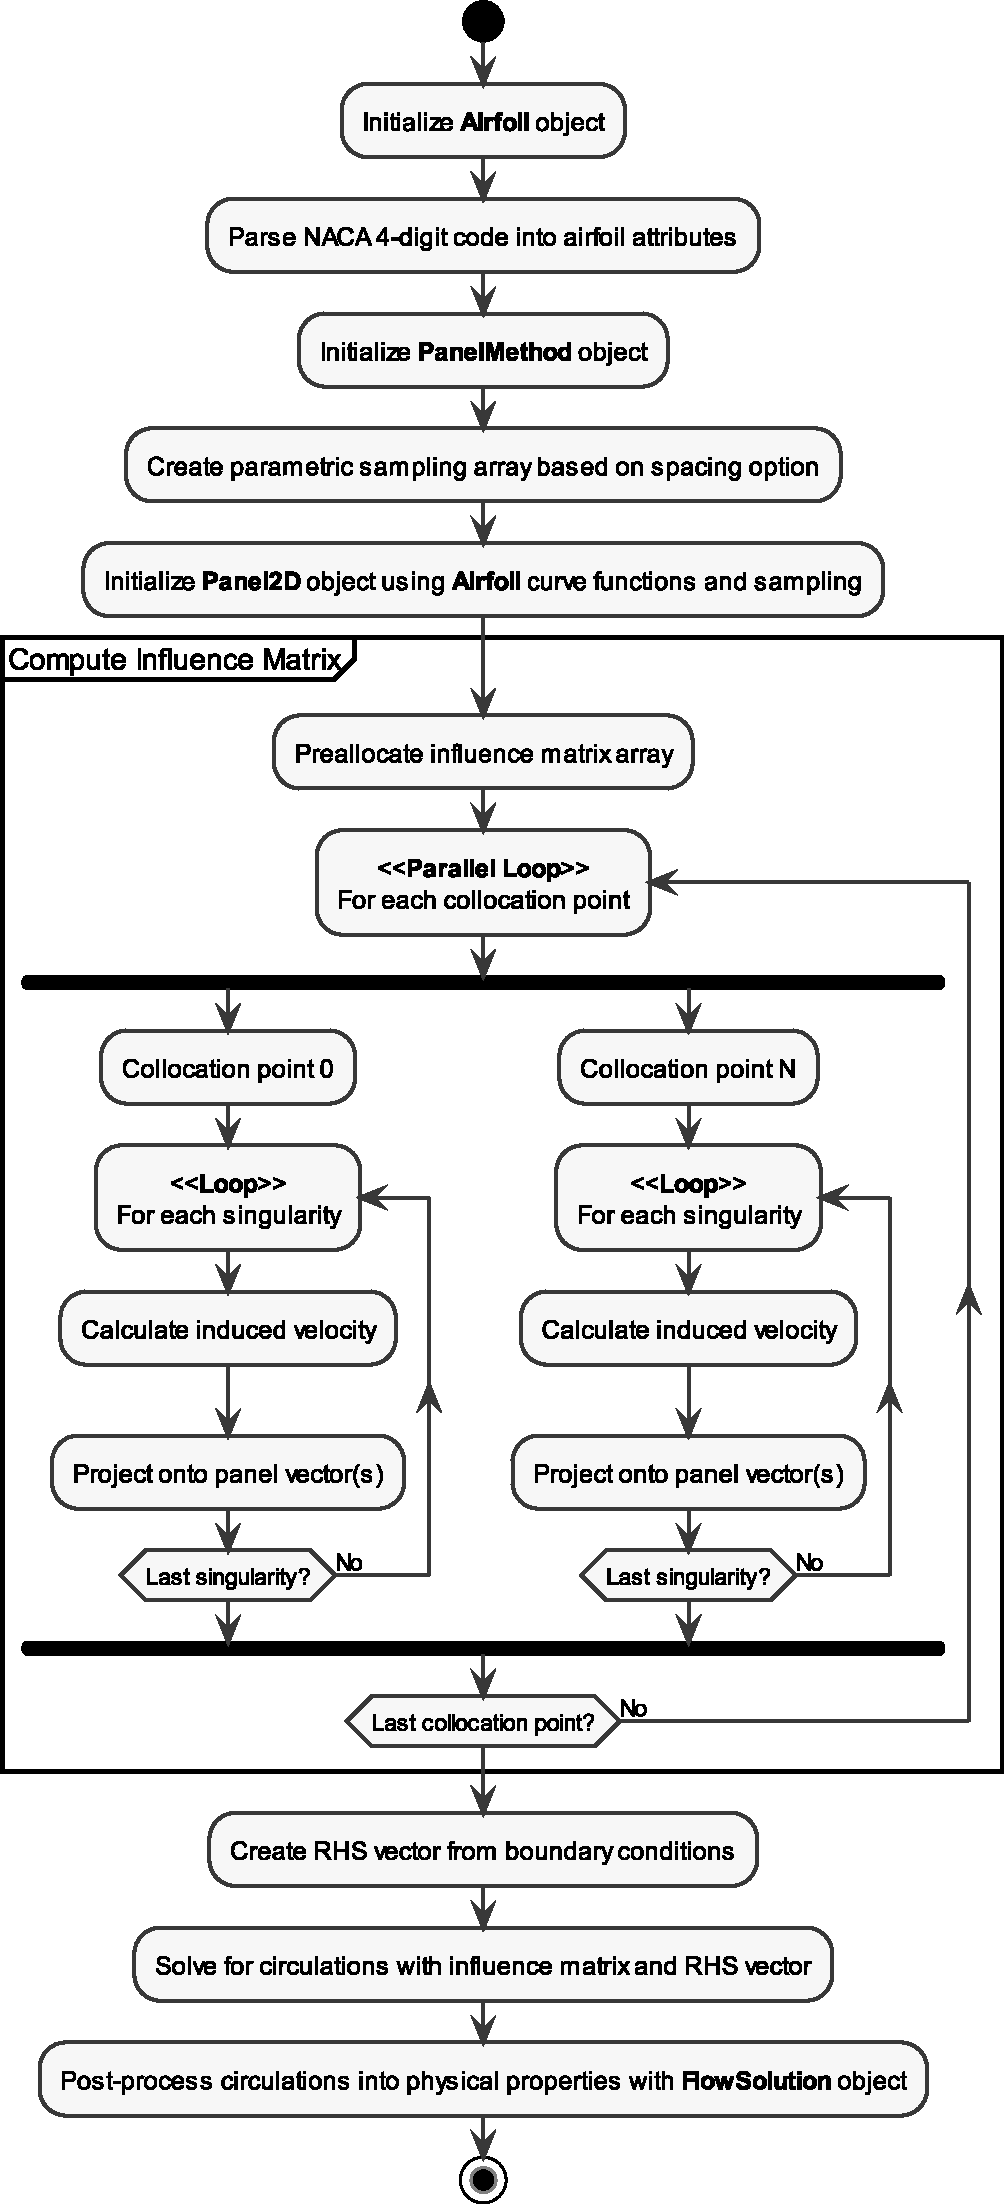
\includegraphics[width=0.40\textwidth]{static/activity_diagram.pdf}
    \end{center}
    \caption{UML Activity Diagram of \numfoil}
    \label{fig:activity}
\end{wrapfigure}

\blindtext\\

\blindtext\\

\section{Geometry Definition}
Before we can begin the analysis, the functions describing the desired airfoil's
camber line, and upper and lower surface should be created. Airfoils are defined
using the NACA 4-digit code. \autoref{eq:camber} is used to obtain the camber
line function.

\begin{equation}
\label{eq:camber}
    y_{c}=\left\{
        \begin{array}{ll}
            \frac{m}{p^{2}}\left(2 p\left(\frac{x}{c}\right)-\left(\frac{x}{c}\right)^{2}\right),
            & 0 \leq x \leq p c \\
            \frac{m}{(1-p)^{2}}\left((1-2 p)+2 p\left(\frac{x}{c}\right)-\left(\frac{x}{c}\right)^{2}\right),
            & p c \leq x \leq c
        \end{array}\right.
\end{equation}
\medskip

Here $m$ is the maximum camber and $P$ is the location of the maximum camber, or
the first and second digit of the 4-digit NACA code divided by ten respectively.
Subsequently, to find the coordinates of the the upper and lower airfoil
surface, the thickness is applied perpendicular to the camber line using
\autoref{eq:coor_u} and \autoref{eq:coor_l} respectively, where $\theta =
\arctan\left( \frac{y_c}{dx}\right)$.

\begin{equation}
\label{eq:coor_u}
    \left(\begin{array}{l} x_U, \: y_U\end{array}\right) =
    \left(\begin{array}{l} x-y_t \sin \theta, \: y_c+y_t\cos \theta\end{array}\right)
\end{equation}
\begin{equation}
\label{eq:coor_l}
    \left(\begin{array}{l} x_L, \:  y_L\end{array}\right) =
    \left(\begin{array}{l} x+y_t \sin \theta, \: y_c-y_ t \cos \theta\end{array}\right)
\end{equation}

\chapter{Panel Methods}  % TODO Decide if this should be a section?
Two different methods well be implemented to peform basic airfoil analysis.
First, the airfoil is represented by its camberline only, and thus has a
thickness of zero. The results of this method will be compared with the second
method, which discritizes the airfoil by placing panels on the outer surface
instead. Hence this second method does take airfoil thickness into account.

\section{Lumped Vortex Method}
\label{sec:thin}
The first method, described by \citeauthor{katz_plotkin}\cite{katz_plotkin}, analyzes an airfoil
looking only at the airfoil's camber line. This discritization is visualized in
\autoref{fig:discr_thin}, where $n=7$ panels are placed on the camber line starting at
the leading edge. These panels are created by adding $n+1$ nodes on the camber
line, the coordinates for which are obtained using the camber line function from
\autoref{eq:camber}. Lumped vortex elements and collocation points are placed at
25\% and 75\% of each panel's length. This way the airfoil is represented as a
set of zero-thickness vortex sheets. Not that linear node spacing is used in
\autoref{fig:discr_thin}. For the implementation, however, cosine spacing is used to
increase accuracy of the results at the leading and trailing edge.


\begin{figure}[H]
\centering
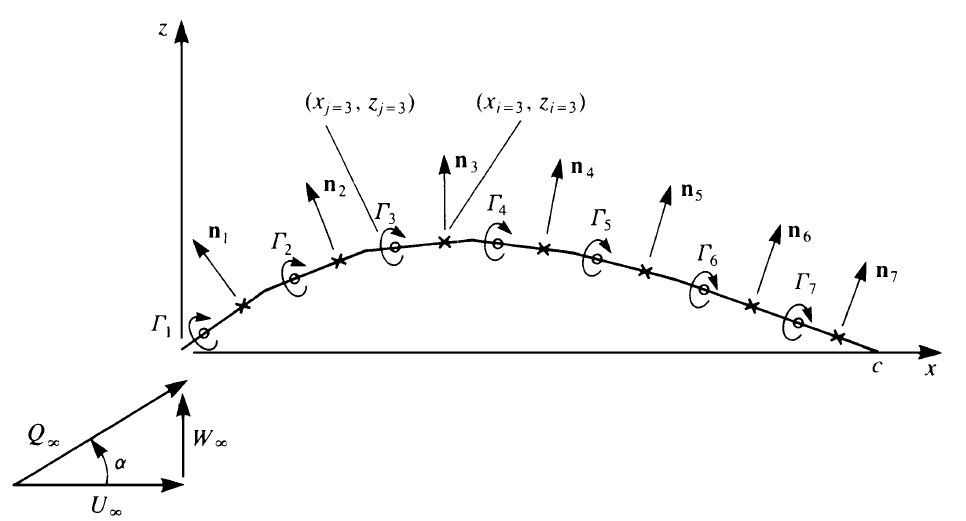
\includegraphics[width=.8\textwidth]{static/disc_camber.png}
\caption{Discritization of the airfoil camber line using $n=7$ panels \cite{katz_plotkin}}
\label{fig:discr_thin}
\end{figure}

\subsection{Equations}
The normal velocity, which consists of the free-stream velocity and the
self-induced velocity, must be zero at each point along the camber line. This
way the camber line is set to be a streamline of the free-stream. This
boundary condition is described by \autoref{eq:thin_cond}. Here,
$\vec{\bf{n}}_i$ is the normal vector of the $i-$th panel given by
\autoref{eq:normal}, and $\alpha_i$ is the angle w.r.t. the x-axis of the $i-$th
panel.

\begin{equation}
\label{eq:thin_cond}
    \left( u_i, \: w_i \right) \cdot \vec{\bf{n}}_i + \left( U_\infty,
    \: W_\infty \right) \cdot  \vec{\bf{n}}_i = 0
\end{equation}
\begin{equation}
\label{eq:normal}
    \vec{\bf{n}}_i = \left( \sin \alpha_i, \: \cos \alpha_i \right)
\end{equation}

Next, if $\left( x_i, \: y_i \right)$ is the location of the $i-$th panel
collocation point, and $\left( x_j, \: y_j \right)$ is the location of the
$j-$th vortex element, the velocity induced at each collocation point due to
the presence of the $n$ vortices, with strength $\Gamma_j$, is found using
\autoref{eq:v_ind_thin}. Note that an error exists within the textbook, as to
represent a correct induced velocity due to the $j-$th vortex element which are
clock-wise rotating, a clock-wise affine transform must be used. Originally, a
counter-clockwise affine transform is provided in \cite{katz_plotkin}.
\medskip

\begin{equation}
\label{eq:v_ind_thin}
    \left(\begin{array}{l}
    u_i \\ w_i
    \end{array}\right)
    =
    \sum_{j=1}^{n} \:
    \left[ \frac{\Gamma_{j}}{2 \pi r_{i,j}^{2}}
    \left(\begin{array}{cc}
    0 & -1 \\ 1 & 0
    \end{array}\right)
    \left(\begin{array}{l}
    x_i-x_{j} \\ z_i-z_{j}
    \end{array}\right) \right], \; \; \; \; \; \forall \; i \in \{1,...,n\}
\end{equation}
\begin{equation}r_{j}^{2}=\left(x_i-x_j\right)^{2}+\left(z_i-z_j\right)^{2}\end{equation}
\medskip

Naturally, if $i=j$, the respective collocation point and vortex are located
on the same panel. The vorticities, $\Gamma_j$, are the unknown which will be solved for.
Combining \autoref{eq:v_ind_thin} with \autoref{eq:thin_cond}, and moving the free-stream
velocity from \autoref{eq:thin_cond} to the right hand side of the equation,  yields a
system of $n$ equations which can be solved algebraically to find the vorticity of each vortex element.
Once the vorticity $\Gamma_j$ is know for each vortex element, the change in lift and
pressure are obtained using \autoref{eq:thin_lift} and \autoref{eq:thin_press} respectively.
 $s_i$ is the length of the $i-$th panel.

\begin{equation}
\label{eq:thin_lift}
\Delta L_i = \rho v_\infty \Gamma_{j=i}
\end{equation}
\begin{equation}
\label{eq:thin_press}
\Delta P_i = \rho v_\infty \frac{\Gamma_{j=i}}{s_i}
\end{equation}

\subsection{Verification}
The results of the zero-thickness camberline panel method are verified by
comparison with example data from \citeauthor{katz_plotkin} for an elliptical
camberline with a maximum camber of $0.1$. Since Naca 4-digit airfoils are
limited to a maximum camber of $0.09$, the Naca 9501 is used to approximate that
same airfoil. Both the reference plot and obtained plot are shown in \autoref{fig:verif_thin}.

% ###########################################################################################
% ###########################################################################################

\section{Linear Vortex Model}
\label{sec:thick}
The second method, described by %\citeauthor{katz_plotkin}\cite{katz_plotkin},
\citeauthor{kuethe_chow_1998}\cite{kuethe_chow_1998}, places vortex elements
with linearly increasing strength in the center of panels on the airfoils
surface. The airfoil is discretized by placing $n$ nodes on the airfoil starting
at the trailing edge, over the lower airfoil surface to the leading edge and
back to the trailing edge over the upper surface. Each node presents a panel
edge, so there are $n-1$ panels. The same naming scheme as used in
\autoref{sec:thin} applies here too.

\subsection{Equations}
\label{ssec:eq_thick}
The boundary condition states that the normal velocity on the panels
must be zero, as described by \autoref{eq:thick_cond}\cite{kuethe_chow_1998}.
The Kutta-condition, shown in \autoref{eq:kutta}, is
added to ensure smooth flow transition to freestream at the trailing edge. This
results in one extra collocation point at the trailing edge, meaning that while
there are only $n-1$ panels, there are $n$ collocation points, the $n$-th one
representing the Kutta-condition.
\begin{equation}
  \label{eq:thick_cond}
  \frac{\partial}{\partial n_{i}} \phi\left(x_{i}, y_{i}\right)=0
  \end{equation}
% \begin{equation}
% \label{eq:thick_cond}
%     \left( U_\infty + u_i, \: W_\infty + w_i \right) \cdot \left( \cos \alpha_i,
%     \: -\sin \alpha_i \right) = 0
% \end{equation}
\begin{equation}
  \label{eq:kutta}
      \gamma_1 + \gamma_{n} = 0
\end{equation}

The velocity potential, $\phi$, in a collocation point at $(x_i,\: y_i)$ due
to $n-1$ vortices located at $(x_j, \: y_j)$ is obtained using
\autoref{eq:phi_thick}.
% When capital letters are used, $(X_j, \: Y_j)$ represent the panel's leading edge
% node, and $(X_{j+1}, \: Y_{j+1})$ refer to the panel's trailing edge node.
% Substituting \autoref{eq:phi_thick} in \autoref{eq:thick_cond} and applying it
% to every collocation point present will yield a system of $n$ equations which
% can be solved for the vorticities $\gamma_j$.


\begin{equation}
  \label{eq:phi_thick}
    \phi\left(x_{i}, y_{i}\right)=V_{\infty}\left(x_{i} \cos \alpha+y_{i} \sin \alpha\right)-\sum_{j=1}^{n-1} \int_{j} \frac{\gamma\left(s_{j}\right)}{2 \pi} \tan ^{-1}\left(\frac{y_{i}-y_{j}}{x_{i}-x_{j}}\right) d s_{j}
  \end{equation}
  \begin{equation}
    \gamma\left(s_{j}\right)=\gamma_{j}+\left(\gamma_{j+1}-\gamma_{j}\right) \frac{s_{j}}{S_{j}}
    \end{equation}
% \begin{equation}
% \label{eq:v_ind_thick}
%     \left(\begin{array}{l}
%     u_{p_i} \\ w_{p_i}
%     \end{array}\right)
%     =
%     \sum_{j=1}^{n} \:
%     \left(\begin{array}{c}
%     \frac{\gamma_j}{2\pi}\left[ \tan^{-1} \left(
%         \frac{z_i - z_{j+1}}{x_i - x_{j+1}}\right)
%          - \tan^{-1} \left( \frac{z_i - z_j}{x_i - x_j}\right) \right] \\[1em]
%     -\frac{\gamma_j}{4\pi} \ln \left[ \frac{\left( x_i - x_j \right)^2 +
%     \left( z_i - z_j \right)^2}{\left( x_i - x_{j+1}\right)^2 +
%     \left( z_i - z_{j+1} \right)^2 }  \right]
%     \end{array}\right), \; \; \; \; \; \forall \; i \in \{1,...,n\}
% \end{equation}
\medskip

% Once that the results of \autoref{eq:v_ind_thick} are in the local panel
% coordinate system and must be transformed back to the global one. Adding
% \autoref{eq:kutta} to the system of equations obtained from
% \autoref{eq:v_ind_thick}, will result in n+1 equations.
% \citeauthor{katz_plotkin}\cite{katz_plotkin} deals with this by replacing an
% arbitrary equation from the system with the Kutta condition, while
% \citeauthor{kuethe_chow_1998}\cite{kuethe_chow_1998} adds an equation, where the
% Kutta condition is altered as shown in \autoref{eq:kutta2}. Either way results
% in again an equal amount of equations and unknowns.
% \begin{equation}
%   \label{eq:kutta2}
%       \gamma_1 + \gamma_{n+1} = 0
% \end{equation}

Finally, \cref{eq:vind_thick} can be used to determine the induced velocity on a
panel due to all vortices present on the surface panels. For the details of this
linear vortex method and a simplified way to implement it by splitting up and
replacing large and complex equations with multiple coefficients
\citeauthor{kuethe_chow_1998}\cite{kuethe_chow_1998}
.
\begin{equation}
  \label{eq:vind_thick}
  V_{i}=\cos \left(\theta_{i}-\alpha\right)+\sum_{j=1}^{n} A_{i j} \gamma_{j}^{\prime}
  \end{equation}


Once the vorticity $\gamma_j$ is known for each vortex element, the change in
lift and pressure are obtained using \autoref{eq:thick_lift}, where
$\vec{\bf{L}}_i$ is the lift direction obtained by rotating the free stream
vecor by \SI{90}{\degree} and
\autoref{eq:thick_press} respectively.

\begin{equation}
\label{eq:thick_lift}
\sum_{i=1}^{n} C_{p_i} s_i \vec{\bf{n}}_i \cdot \vec{\bf{L}}
\end{equation}
\medskip
\begin{equation}
\label{eq:thick_press}
C_{p_i} = 1 - v_i^2
\end{equation}
\medskip

% To facilitate the implementation of \autoref{eq:v_ind_thick}, the coefficient
% breakdown version by \citeauthor{kuethe_chow_1998} was used in the actual code
% for this problem.

\subsection{Verification}
The linear vortex method with paneled airfoil surface is validated with data
obtained from XFOIL\cite{xfoil}. The pressure distribution found for two
different airfoils is shown in \autoref{fig:thick_verif}.
\autoref{fig:thick_verif1}  shows the results for
the NACA0015 at 5 degrees angle of attack, while \autoref{fig:thick_verif2} plots results for
the NACA2422 at 10 degrees angle of attack. Both have the respective results
obtained from XFOIL plotted on top of the results obtained with \numfoil. It can be seen
that the results coincide almost perfectly, with only negligible differences
observable at the suction peak on the upper surface leading edge.

\begin{figure}[h]
    \centering
    \begin{subfigure}{.5\textwidth}
      \centering
      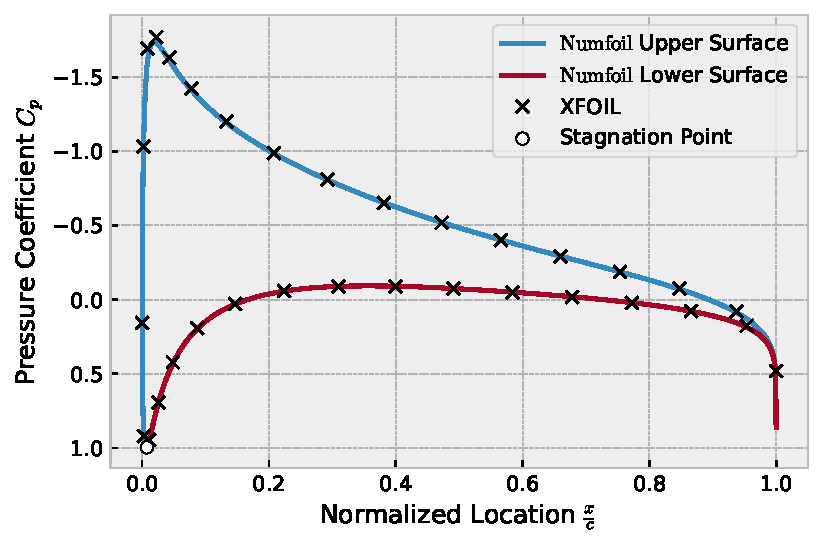
\includegraphics[width=.9\linewidth]{static/thick_verif_naca0015_alpha5.pdf}
      \caption{Pressure distribution NACA0015 at $\alpha = 5^{\circ}$}
      \label{fig:thick_verif1}
    \end{subfigure}%
    \begin{subfigure}{.5\textwidth}
      \centering
      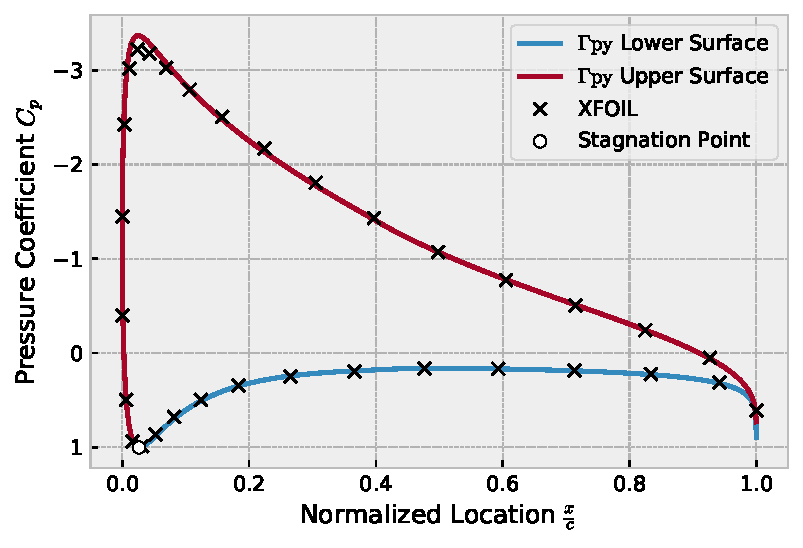
\includegraphics[width=.9\linewidth]{static/thick_verif_naca2422_alpha10.pdf}
      \caption{Pressure distribution NACA2422 at $\alpha = 10^{\circ}$}
      \label{fig:thick_verif2}
    \end{subfigure}
    \caption{\centering Validation of linear vortex method results with XFOIL\cite{xfoil}}
    \label{fig:thick_verif}
\end{figure}


Looking at the resulting estimation for $C_l$, shown in \autoref{tab:cl_thick},
it can be seen that the calculated values for the lift coefficient are slightly
below the values returned by XFOIL. For the NACA0012, the relative error
$\epsilon$ is zero for $\alpha=0$, and increases with angle of attack. When
$\alpha=10\deg$, the error has risen to $\epsilon=-3.51\%$ (the minus indication
the obtained values is lower than the one returned by XFOIL). The same is true
for the NACA4412 results, where the error $\epsilon$ is lowest when $\alpha$ is
zero, and increases with increasing angle of attack. The value of the error si
lower, however, than for the symmetrical airfoil, having a value of
$\epsilon=-2.07\%$ at $\alpha=10\deg$. These results are also shown as plots in \autoref{fig:cl_thick}

\begin{table}[H]
	\centering
	\caption{Estimated values of $C_l$ for a range of angles of attack from XFOIL and NumFoil, as well as the relative error, for NACA0012 and NACA4412.}
	\label{tab:cl_thick}
    \begin{tabularx}{\textwidth}{C  C C C | C C C} %'L' for Left Aligned, 'C' for Centered, 'R' for Right Aligned
    \toprule\
    \hfill & \multicolumn{3}{c}{$C_l$ NACA0015} & \multicolumn{3}{c}{$C_l$ NACA2422} \\ \toprule
    {$\alpha \:[\deg]$} & {$NumFoil$} & {$XFOIL$} & {$\epsilon$} & {$NumFoil$} & {$XFOIL$} & {$\epsilon$} \\ \toprule
    0   & 0        & 0      & 0         & 0.2868 & 0.2742  & +0.0126    \\ \hdashline
    3   & 0.3687   & 0.3708 & -0.0021   & 0.6745 & 0.6645  & +0.0100    \\ \hdashline
    5   & 0.6140   & 0.6175 & -0.0035   & 0.9320 & 0.9238  & +0.0082    \\ \hdashline
    8   & 0.9802   & 0.9861 & -0.0059   & 1.3159 & 1.3105  & +0.0054    \\ \hdashline%\midrule
    10  & 1.2227   & 1.2304 & -0.0077   & 1.5698 & 1.5663  & +0.0035    \\ \hdashline
    13  & 1.5834  & 1.5939 & -0.0105   & 1.9468 & 1.9464  & +0.0004     \\ \bottomrule
    \end{tabularx}
\end{table}

\begin{figure}[h]
  \centering
  \begin{subfigure}{.5\textwidth}
    \centering
    \captionsetup{width=.8\linewidth}
    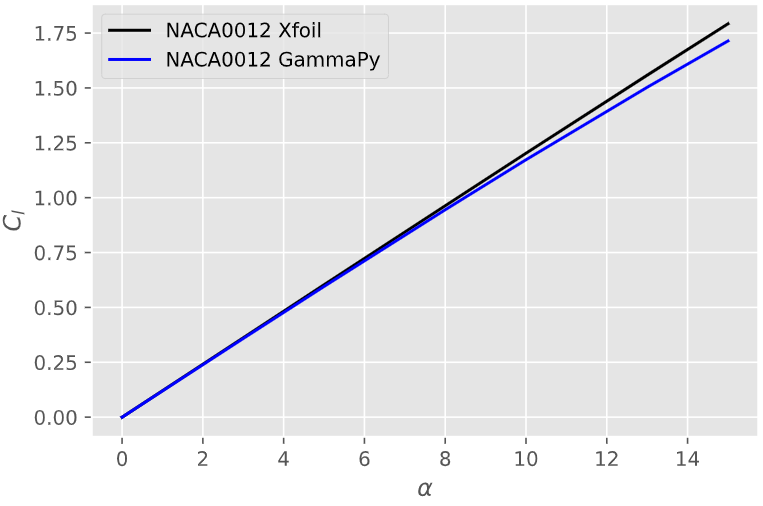
\includegraphics[width=.9\linewidth]{static/naca0012_cl_verif.png}
    \caption{\centering $C_l - \alpha$ plots for NACA0012}
    \label{fig:cl_thick_0012}
  \end{subfigure}\hfill% or \hspace{5mm} or \hspace{0.3\textwidth}
  \begin{subfigure}{.5\textwidth}
    \centering
    \captionsetup{width=.9\linewidth}
    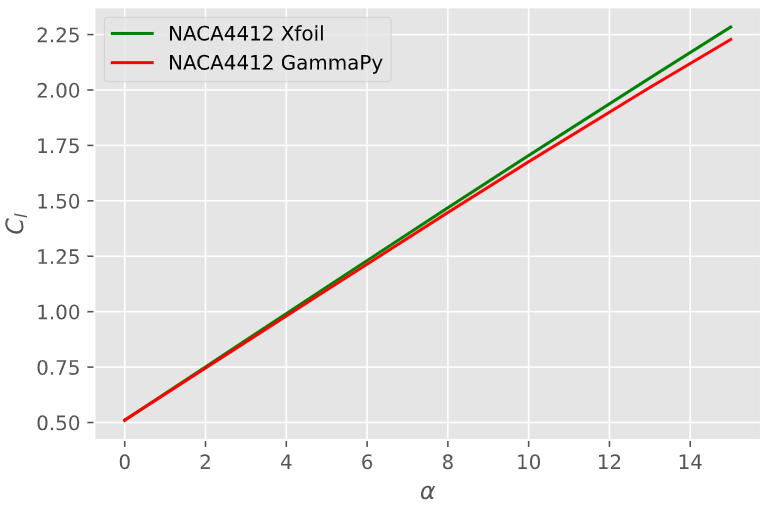
\includegraphics[width=.9\linewidth]{static/naca4412_cl_verif.png}
    \caption{\centering $C_l - \alpha$ plots for NACA0012}
    \label{fig:cl_thick_4412}
  \end{subfigure}
  \caption{\centering Comparing  $C_l - \alpha$ with results from XFOIL for NACA0012 and NACA4412}
  \label{fig:cl_thick}
\end{figure}

% ###########################################################################################
% ###########################################################################################
\chapter{Analysis}
Now that the program is validated, the different aspects of airfoils can be
looked at. First, the effect of camber is discussed in \autoref{sec:camber}.
Next, the change in results due to varying panel thickness is evaluated in
\autoref{sec:thickness}, and, finally, the effect of panel density on the
obtained results is checked in \autoref{sec:panels}.

\section{Effect of Camber}
\label{sec:camber}
To see the effect of varying camber on the results, both the panelled
comaberline and panelled surface methods will be used on airfoils a set of
airfoils (see \autoref{fig:camber}) where the only the camber value is
different. The first one, NACA0012, is a symmetrical airfoil and thus has zero
camber. Subsequent airfoils NACA2412, NACA4412, and NACA9412 have a respective
maximum camber of 0.2, 0.4, and 0.9 at $\frac{x}{c}=0.4$. \autoref{fig:camber1}
plot these airfoils' pressure distributions for $\alpha=3$, and
\autoref{fig:camber2} does the same for $\alpha=8$.

\begin{figure}[h]
    \centering
    \begin{subfigure}{.5\textwidth}
      \centering
      \captionsetup{width=.8\linewidth}
      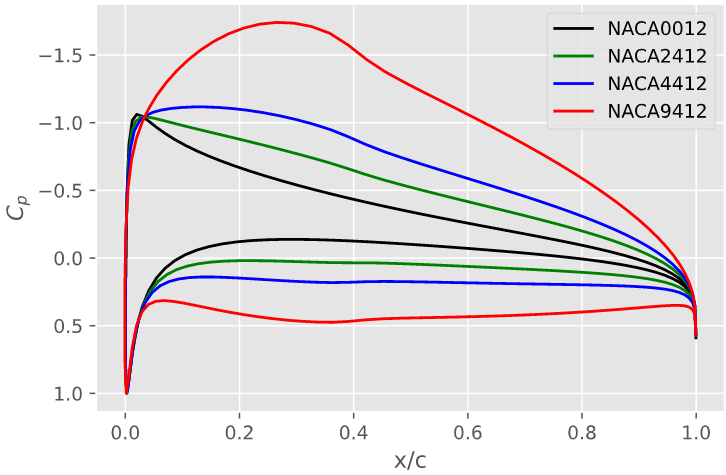
\includegraphics[width=.9\linewidth]{static/camber_a3.png}
      \caption{\centering Pressure distributions with varying camber at $\alpha = 3^{\circ}$}
      \label{fig:camber1}
    \end{subfigure}\hfill% or \hspace{5mm} or \hspace{0.3\textwidth}
    \begin{subfigure}{.5\textwidth}
      \centering
      \captionsetup{width=.9\linewidth}
      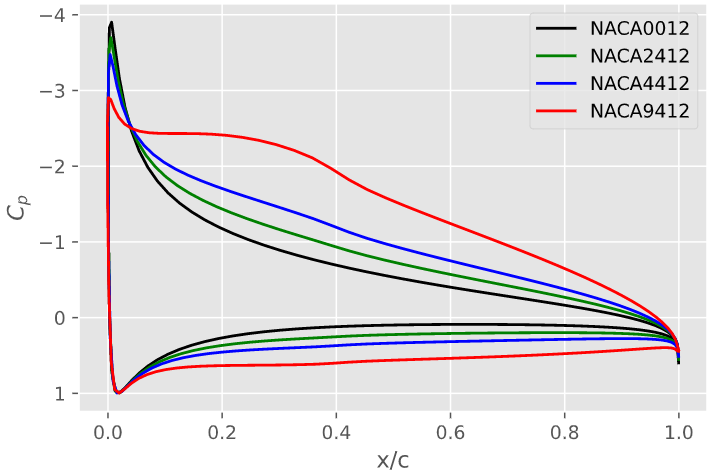
\includegraphics[width=.9\linewidth]{static/camber_a8.png}
      \caption{\centering Pressure distributions with varying camber at $\alpha = 8^{\circ}$}
      \label{fig:camber2}
    \end{subfigure}
    \caption{\centering Plots showing the effect of camber on the pressure distribution}
    \label{fig:camber}
\end{figure}

Clearly, a higher camber value leads to higher local values for the pressure
coefficient. This means the plotted lines representing the $C_p$ of the upper
and lower surfaces lie further appart. This increase in pressure difference in
turn results in a higher value for the lift coefficients. The increase of $C_P$
with camber is not linear. It can be seen that at high values for camber, the
increase of pressure coefficients with camber is higher than for low camber.

The same is true for $C_l$, as shown in \autoref{fig:cambercl}. For different
angles of attack, the $C_l$ is plotted as a function of camber for two airfoil
series: \autoref{fig:cambercl1} shows the $C_l$ variations for NACA4X12, where X
is the camber value$x10$, and \autoref{fig:cambercl2} shows the $C_l$ variations
for NACA2X22. Angle of attack clearly has no effect on how much the camber
increases the lift coefficient, as the lines of different values for $\alpha$
ahave equal gradients for every camber value.

\begin{figure}[h]
    \centering
    \begin{subfigure}{.5\textwidth}
      \centering
      \captionsetup{width=.8\linewidth}
      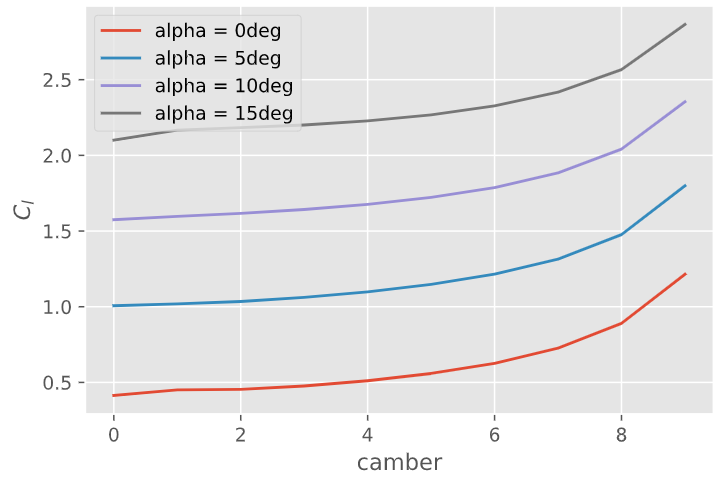
\includegraphics[width=.9\linewidth]{static/cambereffect_thick.png}
      \caption{\centering Variation of $C_l$ with camber for NACA4X12}
      \label{fig:cambercl1}
    \end{subfigure}\hfill% or \hspace{5mm} or \hspace{0.3\textwidth}
    \begin{subfigure}{.5\textwidth}
      \centering
      \captionsetup{width=.9\linewidth}
      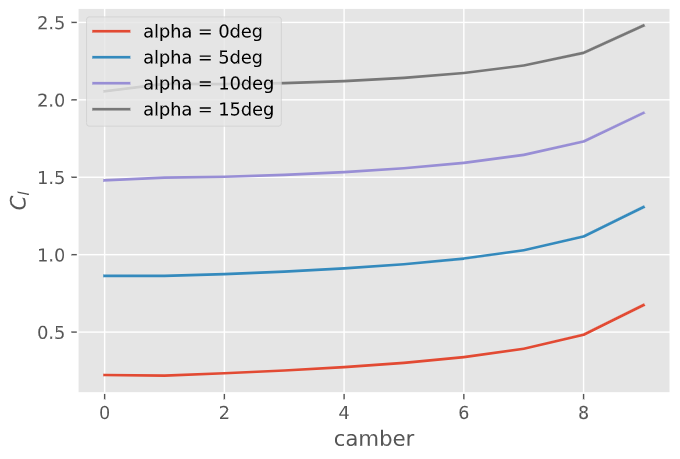
\includegraphics[width=.9\linewidth]{static/cambereffect2_thick.png}
      \caption{\centering Variation of $C_l$ with camber for NACA2X22}
      \label{fig:cambercl2}
    \end{subfigure}
    \caption{\centering Variation of $C_l$ with increasing camber for different angles of attack. The X in the NACA codes is the camber which is varied.}
    \label{fig:cambercl}
\end{figure}



\section{Effect of Airfoil Thickness}
\label{sec:thickness}

For the lumped vortex method, with a panelled camberline, as discussed in
\autoref{sec:thin}, the thickness will not have any effect on the results. This
method only looks at the camberline, and ignores the airfoil's thickness.
Instead, only the constant vortex method with panelled airfoil surfaces from
\autoref{sec:thick} can be used for this. Again, results for symmetric
(NACA00XX) and cambered airfoils (NACA44XX) are plotted in
\autoref{fig:thickcp1} and \autoref{fig:thickcp2} respectively. The angle of
attack is constant for all cases: $\alpha = 5^{\circ}$. The pressure
distributions show that an increase in thickness reduces the suction peak on the
leading edge, while increasing the pressure deferential over the rest of the
airfoil, leading to a net increase in lift. This is confirmed by looking at the
change of $C_l$ with increasing thicness, shown in \autoref{fig:thickcl}.
Comparing the results for a symmetric airfoil (\autoref{fig:thickcl1}) with
those for a cambered airfoil (\autoref{fig:thickcl2}), shows that the increase
in lift for a cambered airfoil is greater than for a symmetric airfoil if the
thickness is increased. This can be seen by the slightly larger gradients in
\autoref{fig:thickcl2}, compared to \autoref{fig:thickcl1}.

\begin{figure}[h]
  \centering
  \begin{subfigure}{.5\textwidth}
    \centering
    \captionsetup{width=.8\linewidth}
    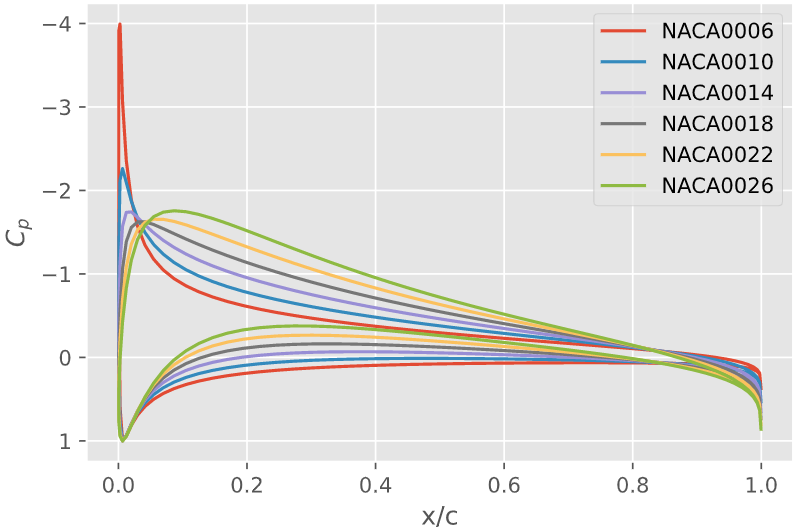
\includegraphics[width=.9\linewidth]{static/thickness_effect_00xx.png}
    \caption{\centering Pressure distributions with varying thickness for a symmetric airfoil}
    \label{fig:thickcp1}
  \end{subfigure}\hfill% or \hspace{5mm} or \hspace{0.3\textwidth}
  \begin{subfigure}{.5\textwidth}
    \centering
    \captionsetup{width=.9\linewidth}
    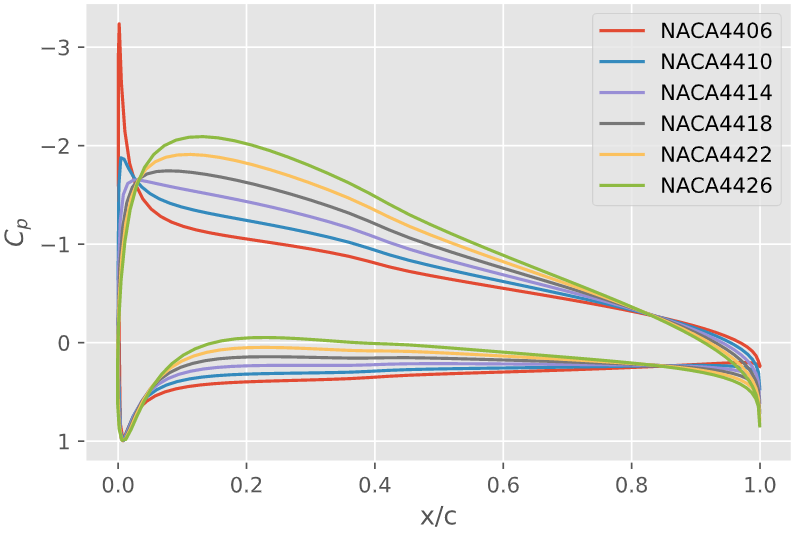
\includegraphics[width=.9\linewidth]{static/thickness_effect_44xx.png}
    \caption{\centering Pressure distributions with varying thickness for a cambered airfoil}
    \label{fig:thickcp2}
  \end{subfigure}
  \caption{\centering Effect of thickness on the pressure distribution for a cambered and symmetric airfoil at $\alpha = 5^{\circ}$.}
  \label{fig:thickcp}
\end{figure}

\begin{figure}[h]
  \centering
  \begin{subfigure}{.5\textwidth}
    \centering
    \captionsetup{width=.8\linewidth}
    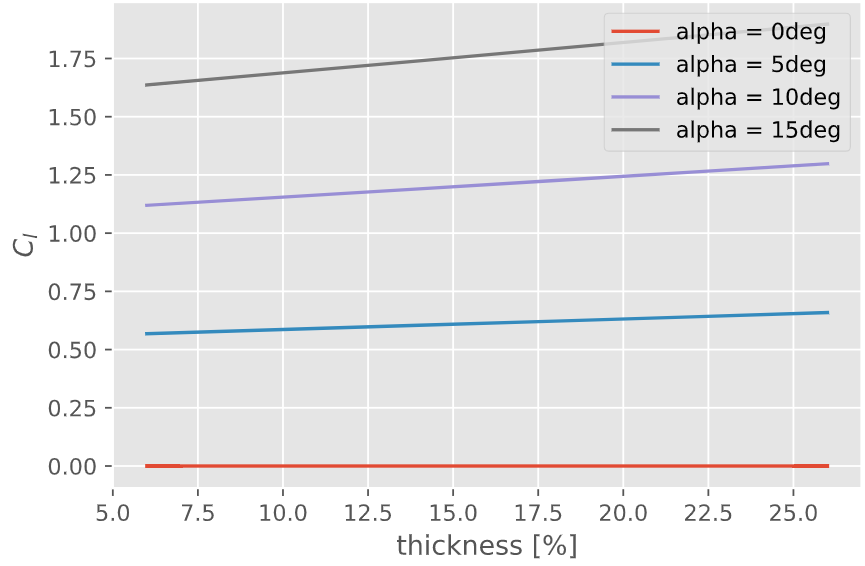
\includegraphics[width=.9\linewidth]{static/thickness_Cl_effect_00xx.png}
    \caption{\centering $C_l$ values for varying thickness for a symmetric airfoil (NACA00XX)}
    \label{fig:thickcl1}
  \end{subfigure}\hfill% or \hspace{5mm} or \hspace{0.3\textwidth}
  \begin{subfigure}{.5\textwidth}
    \centering
    \captionsetup{width=.9\linewidth}
    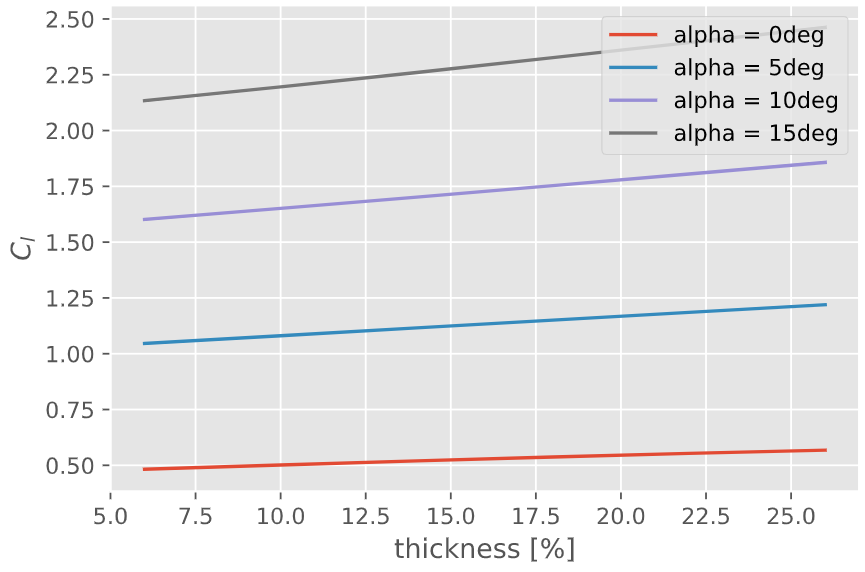
\includegraphics[width=.9\linewidth]{static/thickness_Cl_effect_44xx.png}
    \caption{\centering $C_l$ values for with varying thickness for a cambered airfoil (NACA44XX)}
    \label{fig:thickcl2}
  \end{subfigure}
  \caption{\centering Effect of thickness on the $C_l$ for a cambered and symmetric airfoil at different angles of attack.}
  \label{fig:thickcl}
\end{figure}



\section{Effect of Panel Density}
\label{sec:panels}
Varying the panel density of course will also vary the fidelity of the analysis.
\autoref{fig:thick_panels} shows the effect of increasing the amount of panels
on $C_l$ (with $\alpha = 5^{\circ}$), for a symmetric (\autoref{fig:thick_panels1}) and a cambered
(\autoref{fig:thick_panels2}) airfoil. The choice was made to consider values
with a relative error lower than 0.5\%, compared to values from XFOIL, are
adequate. To satisfy this requirement, 98 panels are needed for the symmetric
airfoil and 102 are required for the cambered airfoil. From this it can be
concluded that, to obtain adequately accurate values, at no less than 100 panels
should be used at all times.

\begin{figure}[h]
  \centering
  \begin{subfigure}{.5\textwidth}
    \centering
    \captionsetup{width=.8\linewidth}
    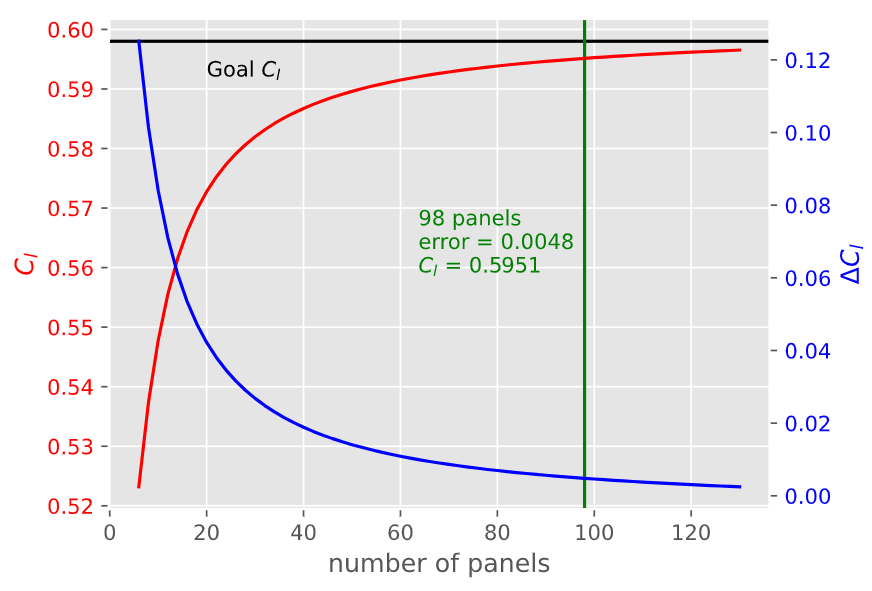
\includegraphics[width=.9\linewidth]{static/conv_thick_sym.png}
    \caption{For the NACA0012 at $\alpha = 5^{\circ}$, results are within 0.5\% of XFOIL with 98 panels}
    \label{fig:thick_panels1}
  \end{subfigure}%
  \begin{subfigure}{.5\textwidth}
    \centering
    \captionsetup{width=.8\linewidth}
    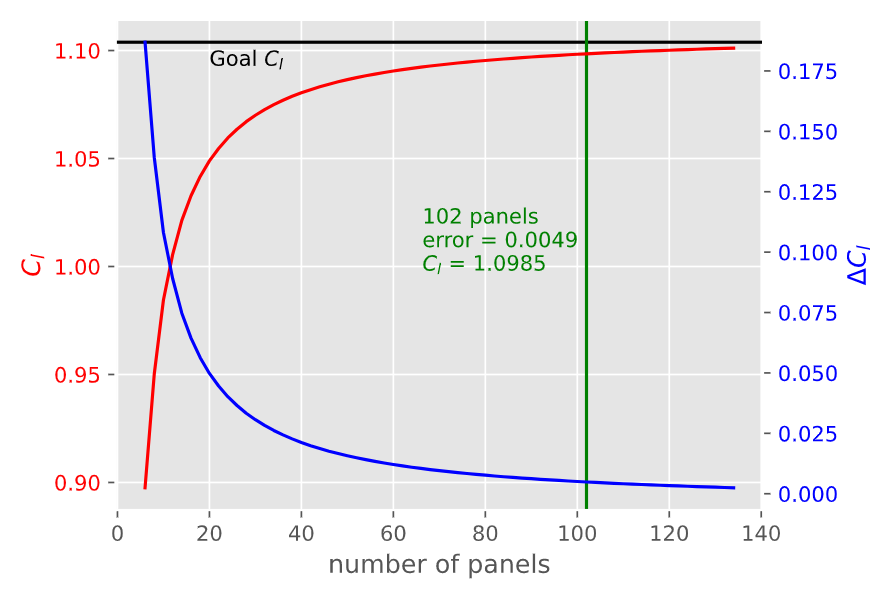
\includegraphics[width=.9\linewidth]{static/conv_thick.png}
    \caption{For the NACA4412 at $\alpha = 5^{\circ}$, results are within 0.5\% of XFOIL with 102 panels}
    \label{fig:thick_panels2}
  \end{subfigure}
  \caption{\centering Convergence of results with increasing panel density}
  \label{fig:thick_panels}
\end{figure}
